% Szablon przygotowany przez Jarosława Drapałę z dalszymi zmianami Michała Karola

% Sprawozdanie max 4 strony A4
% Repozytorium kodu powinno być dostępne przez prowadzącego
% Zalecane środowisko: Overleaf

\documentclass[10pt]{article}

\usepackage{polski}
\usepackage{graphicx}
\usepackage{hyperref}
\graphicspath{{images/}}

\usepackage{geometry}
\newgeometry{tmargin=4cm, bmargin=4cm, lmargin=3.2cm, rmargin=3.2cm} 

\usepackage{fancyhdr}
\pagestyle{fancy}

 

\begin{document}

% Szablon przygotowany przez Jarosława Drapałę z dalszymi zmianami Michała Karola

\begin{titlepage}
\begin{center}
  
  \LARGE \textsc{Politechnika Wrocławska}\\
  \vspace*{0.2cm}
  \Large \textsc{Wydział Informatyki i Telekomunikacji}\\  
  \vspace*{0.4cm}
  \centering
\includegraphics[width=0.2\textwidth]{WITlogo.png}\\
  \vspace*{0.2cm}
  \vspace*{2cm}
        
  \centerline{\rule{\textwidth}{1.2pt}}
  \vspace{0.4cm}
  \Huge\textbf{Przewidywania zdobytego złota i obrażeń na podstawie statystyk z gry League of Legends}
  \centerline{\rule{\textwidth}{1.2pt}}
  \vspace{1cm}
  \LARGE Sprawozdanie z laboratorium\\
  \vspace{3cm}
  \textsc{Autor}\\
  \vspace{0.2cm}
  \textbf{Jan Skibiński}\\
  \vspace{0.1cm}
  \Large nr albumu: \textbf{260460}\\
  \vspace{0.1cm}
  kierunek: \textbf{Informatyka stosowana}
            
            
        
        
  \vspace*{\fill}
  \Large \textit{13 czerwiec 2022}
            
 \end{center}


\end{titlepage}

\begin{abstract}
Praca przedstawia system, który pozwala przewidzieć zdobyte złoto/zadane obrażenia w meczu gry Leage of Legends na podstawie statystyk (K/D/A, czas gry, zabite miniony). Dataset został pobrany z użyciem Riot API. Pobrane dane zostały następnie oczyszczone oraz użyto modelu do predykcji zdobytego w meczu złota na podstawie statystyk gracza.

\end{abstract}

\section{Wstęp -- sformułowanie problemu}
\label{sec:wstep}

Autor potrzebuje przewidzieć przewagę złota swoich przeciwników, względem siebie i swojej drużyny w obecnie trwającym meczu. Informacja ta nie jest wyświetlana, dopóki mecz się nie zakończy, a jest to użyteczna informacja, pozwalająca na skuteczniejsze wybieranie celu ataku.

\section{Opis danych}
Wielkość datasetu 100 wierszy. (Zbiór watości jest specyficzny dla datasetu, potencjalnie wszystkie są \textless0, oo))
\newline
Kolumna "kills" - zmienna int, określa ona ilość zabójstw zdobytych przez danego gracza w meczu. Zbiór wartości: $<$1, 22$>$
\newline
Kolumna "deaths" - zmienna int, określa ona ilość zgonów danego gracza w meczu.
\newline
Zbiór wartości: $<$1, 13$>$
\newline
Kolumna "assists" - zmienna int, określa ona ilość asyst zdobytych przez danego gracza w meczu. Zbiór wartości: $<$1, 24$>$
\newline
Kolumna "minions" - zmienna int, określa ona liczbę zabitych minionów przez danego gracza w meczu.
\newline
Zbiór wartości: $<$7, 215$>$
\newline
Kolumna "duration" - zmienna float, określa ona czas trwania meczu (w minutach).
\newline
Zbiór wartości: $<$11, 31)
\newline
Kolumna "gold" - zmienna int, określa ona ilość złota zdobytego przez danego gracza w meczu. Zbiór wartości: $<$6638, 24300$>$
\newline
Kolumna "damage" - zmienna int, określa ona ilość zadanych obrażeń wrogim bohaterom, przez danego gracza w meczu. Zbiór wartości: $<$3254, 75641$>$

\section{Opis rozwiązania}

Dane do datasetu zostaną pobrane ze strony \url{https://eun1.api.riotgames.com}. Dostęp do danych uzyskano za pomocą API. Baza danych została zapisana w postaci ramki danych biblioteki \texttt{Pandas}. Zawiera ona informacje o 100 ostatnich meczach gry League of Legends (tryp arurf) rozegranych przeze mnie. 

Używając metody \textit{Multiple Linear Regression} (MLR) na danych uzyskano model pozwajacy na określenie złota zdobytego przez gracza w obecnie trwającej grze. Jest to dokonywanie przy pomocy modelu, który bierze jako zmienne decyzyjne: zabójstwa, śmierci, asysty, miniony, czas gry i na ich podstawie próbuje przewidzieć, ile złota gracz zdobył w tej grze. Jest to możliwe, dzięki mocnej korelacji naszych danych, wszystkie zmienne decyzyjne wpływają pośrednio lub bezpośrednio na to, ile dany gracz zdobył złota.

\section{Rezultaty obliczeń}

\subsection{Plan badań}
Zbiór danych zostanie podzielony na dwie części: treningową i testową w stosunku, który zwróci najlepsze wyniki (prosta funkcja decyduje o cut poincie, funckja ta jako paremtry przyjmuje minimalny rozmiar danych testowych oraz trainingowych). Przed zdecydowaniem cut pointu usuniemy z danych ekstremalne przypadki (bardzo krótkie mecze)

\subsection{Wyniki obliczeń} 
Model zdobytego złota można określić następującym wzorem:
\begin{equation}
\det Gold = a * kills + b * deaths + c * assists + d * minions + e * duration + f
\label{eq:wzor_wazny}
\end{equation}

Na rys. \ref{fig:korelacje} pokazany jest wykres dopasowania modelu do danych testowych paremetry (MINTEST=16, MINTRAINING=60, MINGAMELENGTH=11). \newline 
\begin{figure}[!hbt]
\begin{center}
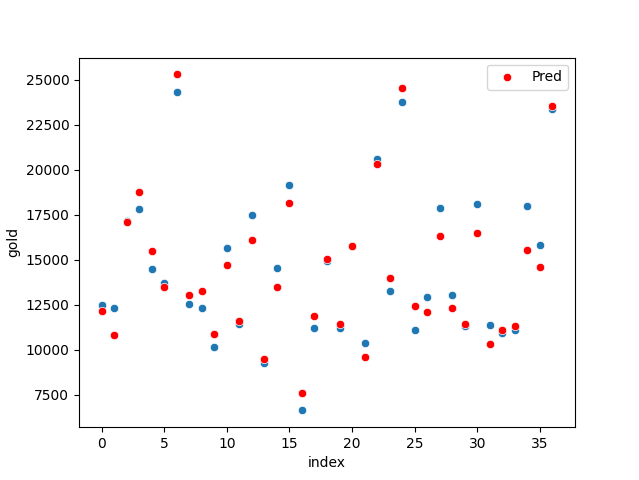
\includegraphics[width=0.8\linewidth]{rys1.png}
\caption{Doposawnie modelu do danych}
\label{fig:korelacje}
\end{center}
\end{figure}


Paramatery wyliczone przez curvefit: a = 415.46962063 b = -26.42115756 c = 140.22010774  d = 34.71285853 e = 377.52246582

Oznacza to, że zgony wpływają negatywnie na zdobyte złoto, natomiast najważniejszymi parametrami są zabójstwa oraz czas gry, zabite miniony będą jako 3 najważniejsze, natomiast asysty nie mają aż tak dużego wpływu.

Podsumowując, symulacje ujawniają że wg. (\ref{eq:wzor_wazny}) wyliczenie złota jaki posiada nasz przeciwnik powinno być relatywnie proste. Starczy zwracać uwagę na czas gry i zabójstwa, oraz zabite miniony, w obliczeniach spokojnie można pominąć asysty i śmierci (chyba, że ma ich bardzo dużo)

Do oceny modelu użyto metryk mean-absolute-error, która wyniosła 756.72 oraz mean-absolute-percentage-error, która wyniosła 5.43\%

\section{Wnioski}
Przedstawiona metoda pozwala na przygotowanie modelu i ten model jest wytrzymały na nowe dane. Uzyskany model daje szczególnie ciekawe dane dla gier o ekstremalnej długości (to znaczy bardzo krótkiej, albo bardzo długiej). Pozwala on zauważyć pewne znaczące zależności od tego, jak statystyki naprawdę wpływają na naszą przewagę w grze. Między innymi pozwala zauważyć, że zgon nie wpływa w znaczący sposób na naszą przewagę, natomiast wpływa on na przewagę przeciwnika.

\appendix
\section{Dodatek}
Kody źródłowe(utrzymane w konwencji języka Python wraz z instrukcjmi uruchomienia) umieszczone zostały w repozytorium github:

\noindent \url{https://github.com/Pandorianim/msid_project}.


\end{document}